\section{Кинематика твердого тела}

\begin{to_def} 
    \textit{Твёрдым телом} назовём множество такое, что
    $$
         \forall i, j, t:
         \hspace{0.5cm} |\vc{r}_i(t) - \vc{r}_j(t)|=\const.
     $$ 
\end{to_def}

Точка $O$ это полюс. Во-первыхх перенесем начало координат в $O$. Введём систему координат $O_{\xi\nu\zeta}$ связанную с телом, -- тело относительно неё не движется.
% \textit{Поступательное движение} -- 
% \textit{Вращательное движение} --
$$
    \vc{r} = \vv{OA}, \, \vc{\rho} = \vv{OA} = \const \text{ в $O_{\xi\nu\zeta}$},
    \hspace{0.5cm} \Rightarrow \hspace{0.5cm} 
    \vc{r}(t) = R(t) \vc{\rho}.
$$
Проведём два вектора $\vc{r}_A, \vc{r}_O$:
$$
    \vc{r}_A = \vc{r}_O + \vc{r} = \vc{r}_O + R(t) \vc{\rho}
    \hspace{0.5cm} \overset{d / dt}{\Rightarrow} \hspace{0.5cm} 
    \vc{v}_A = \vc{v}_O + \dot{R} \rho = \vc{v}_O + \dot{R} R^{-1}\vc{r}
$$
но,
$$
    RR\T = E, \dot{R} R\T + R \dot{R}\T = 0, \dot{R} R\T = - R \dot{R}\T,
    (\dot{R} R^{-1})\T = - \dot{R} R^{-1}.
$$
То есть $\dot{R} R^{-1}$ кососимметрична. Тогда пусть
$$
    \dot{R} R^{-1} = \Omega = \begin{pmatrix}
        0 & -\omega_z & w_y \\
        w_z & 0 & -\omega_x \\
        -\omega_y & \omega_x & 0\\
    \end{pmatrix}
    % матрицу
$$
Тогда можно ввести некоторый оператор, а-ля \textit{угловая скорость}\footnote{
    Определение?
}, и получить
$$
    \vc{v}_A = \vc{v}_O + \vc{\omega} \times \vc{r}
    \hspace{0.5cm} \text{--} \hspace{0.5cm} \text{\textbf{формула Эйлера}.}
$$

\noindent
\textbf{Следствие 1} \\
$$
    \vc{v}_A = \frac{d \vc{a}}{dt} = \vc{\omega} \times \vc{a},
    \hspace{0.5cm} \text{при условии $a = \const$}
$$

\noindent
\textbf{Следствие 2} \\
\begin{align*}
    \vc{w}_A &= \vc{w}_O + \frac{d \vc{\omega}}{dt} \times \vc{r} + \vc{r} \times \frac{d \vc{r}}{dt}, \\
    \vc{w}_A &= \vc{w}_O + \vc{\varepsilon} \times \vc{r} + \vc{\omega} \times \left(\vc{\omega} \times \vc{r} \right)
    \hspace{0.5cm} \text{--} \hspace{0.5cm} \text{\textbf{формула Ривальса},}
\end{align*}
где $\vc{\varepsilon} = d \vc{w} / d t$ -- \textit{угловое ускорение}.

\begin{minipage}[t]{0.45\textwidth}
\begin{align*}
    \text{Точка:} \hspace{0.5cm} 
    \vc{r} \in \mathbb{R}^3, \hspace{0.5cm} n=3 \\
    \vc{v} \\
    \vc{w}
\end{align*}
\end{minipage}
\hfill
\begin{minipage}[t]{0.45\textwidth}
\begin{align*}
    \text{Твёрдое тело:} \hspace{0.5cm} 
    \vc{r}, R \in \mathbb{R}^3 \times SO(3), \hspace{0.5cm} n=6 \\
    \vc{\omega} \\
    \vc{\varepsilon} 
\end{align*}
\end{minipage}

% \subsection{Углы Эйлера}

% \begin{wrapfigure}{r}{0.3\textwidth}
%   \begin{center}
%         \vspace{-10 mm}
%         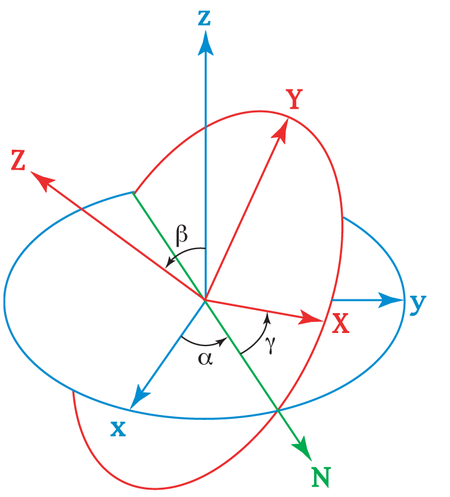
\includegraphics[width=0.9\linewidth]{img/eu_angles.png}
%   \end{center}
%     \caption{Углы Эйлера}
% \end{wrapfigure}

% \begin{align*}
%     1) \hspace{0.25cm}  Oz, \psi &\colon Ox \to ON \\
%     2) \hspace{0.25cm}  Ox, \theta &\colon Oz \to O\xi \\
%     3) \hspace{0.25cm}  O\zeta, \varphi &\colon Ox' \to O\zeta.
% \end{align*}

